\chapter{Selective sequencing}

\label{kap:selSeq} % id kapitoly pre prikaz ref

In this chapter, we are going to describe what is selective sequencing. Then, we
show advantages that this method brings, the main challenges and current state of
research in this area.

\section{DNA sequencing}

One of the goals of biology is ability to obtain DNA sequence of the organism. DNA sequence
is sequence of nucleotides. There are four types of nucleotides: adenin, citozin,
guanin and timin. From now, we will for simplicity assume that DNA sequence is
string of A, C, G, T. The process of obtaining DNA sequence is called DNA sequencing.
One of the devices that serve this purpose is MinION\cite{lu2016oxford}. MinION is a small, cheap and
versatile DNA sequencer. This sequencer consists of a active surface
filled with pores. Pore is a small hole with electric current passing through it. 
As the molecule of DNA is passing through the pore of MinION, we can observe
changes in the flow of an electric current passing through the pore. This electric
current called signal is measured over discrete time. The example of this signal
is on the figure \ref{obr:minIonCurrent}.

\begin{figure}
\centerline{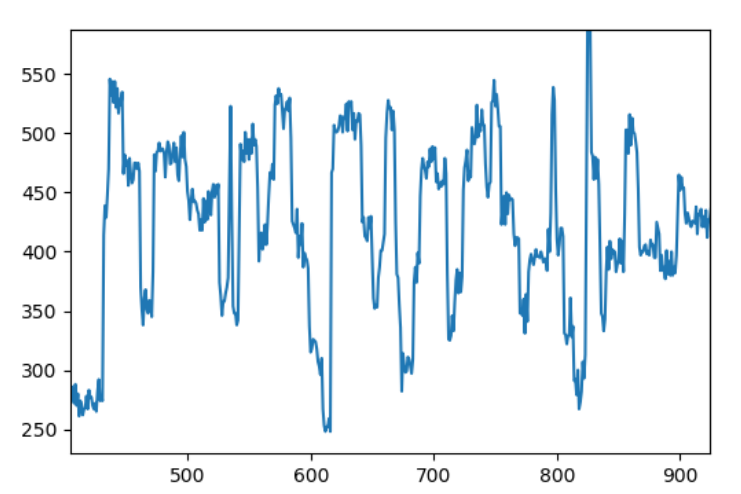
\includegraphics[width=0.7\textwidth, height=0.3\textheight]{images/signal}}
\caption[MinION signal]{Electric current (signal) coming from MinION.}
%id obrazku, pomocou ktoreho sa budeme na obrazok odvolavat
\label{obr:minIonCurrent}
\end{figure}

When we obtain the signal from individual pores, we need to convert it into DNA
sequence. As the molecule of DNA is passing through the pore, only a small
number of nucleotides in the proximity of pore influence the output signal. So from
the signal, using a method called base-calling, we can tell how the molecule of DNA
looked like based on the measurements of signal throughout the time. Despite big
improvements in the base-calling algorithms, the overall process of base-calling
is quite slow and resource-intensive.

\section{Selective sequencing}

Before sequencing, it is convenient to broke down whole DNA molecule into many
shorter parts. We then sequence shorter DNA molecules parallelly. Whole signal
of one shorter DNA molecule is called read.
MinION has one special ability that helps us in certain scenarios. It can reject
DNA molecule that is currently passing
through the pore. It effectively reverses the molecule’s direction and throws it away.
Selective sequencing is the idea that based on the incoming signal, we can tell
if we are interested in sequencing current DNA molecule and can decide if we want
to continue or reject this molecule. This happens on-the-fly so we need to make
the decision until the end of the current read. This means we don't have time to
turn our signal into a nucleotide sequence as the reads are too short. This is
a reason why we have to work with a raw signal.

There are a lot of benefits of selective sequencing. In case we are not interested
in some DNA that we know is contained in our sample, we can use this technique to
reject unwanted DNA molecule. This saves us a lot of time and resources as obtaining
nucleotide sequence from the signal is in some scenarios unnecessary and too
costly process in terms of performance.

Let's say we are trying to find an exact type of virus in human blood. We can
reject all human DNA samples because we are not interested in processing human
DNA. We could also filter in a positive way. So we could say, that we are only
interested in sequencing DNA that produces a signal in some sense similar to our
chosen sample. This all means saving a lot of time and computing power in certain
cases, for example during the disease diagnosis process.

Naturally, there are some drawbacks of selective sequencing. In order to find out
if the currently passing molecule is from human DNA, we have to have some information
about signal from human DNA beforehand.
This is of course in some sense limiting factor as we need a sample signal from
the species that we want to filter. The other problem is that in the case of misclassifying
some signal as not interesting, we lost information about the corresponding
read.

\section{Current state of selective sequencing}
